% -------------------- Result and Analysis ----------------------------------

\pagebreak

\section{Results and Analysis}
%Prepare the test plans in tabular format, where each Test Case should be represented with distinct id, prefixed with “$\langle$module$\rangle$ “, where module represents the short code of the respective design module. Test Case numbers should be matching as stated in Requirement Matrix.
%\vspace{.1in}

%\noindent

%Appropriate definition of ‘Performance Metrics’, e.g. Classification Accuracy, Mean Squared Error etc. should be included, as applicable. 
%\vspace{.1in}

%\noindent
%Depending on your specific project, test results can be represented as a table of data with a corresponding pie chart / bar chart as needed. Analysis of test results should be discussed in terms of clear bullet points.

\noindent
The metrics used for evaluating the performance of the classification models include Precision, Recall, F1-Score, and Support, along with the Confusion Matrix. These metrics are crucial for assessing how well the models are able to differentiate between various classes, providing insight into their accuracy, ability to capture relevant instances, and the overall balance between precision and recall. By analyzing these metrics, a comprehensive understanding of the model's performance can be obtained, enabling informed decisions for further optimization and tuning.

\subsection{Classification Metrics and Confusion Matrix}

\begin{itemize}
    \item \textbf{Precision:} Precision is the ratio of correctly predicted positive observations to the total predicted positives. It can be calculated as:
    \[
    \text{Precision} = \frac{TP}{TP + FP}
    \]
    where \( TP \) represents True Positives, and \( FP \) represents False Positives.

    \item \textbf{Recall:} Recall is the ratio of correctly predicted positive observations to all observations in the actual class:
    \[
    \text{Recall} = \frac{TP}{TP + FN}
    \]
    where \( TP \) is True Positives, and \( FN \) is False Negatives.

    \item \textbf{F1-Score:} F1-Score is the harmonic mean of Precision and Recall, calculated as:
    \[
    \text{F1-Score} = 2 \times \frac{\text{Precision} \times \text{Recall}}{\text{Precision} + \text{Recall}}
    \]

    \item \textbf{Support:} Support refers to the number of actual occurrences of each class in the dataset:
    \[
    \text{Support} = \text{Number of samples in the true class}
    \]

    \item \textbf{Confusion Matrix:} A confusion matrix is used to evaluate the performance of a classification model. It is structured as follows:
    \[
    \begin{bmatrix}
    TP & FP \\
    FN & TN
    \end{bmatrix}
    \]
    where:
    \begin{itemize}
        \item \( TP \) = True Positives
        \item \( FP \) = False Positives
        \item \( FN \) = False Negatives
        \item \( TN \) = True Negatives
    \end{itemize}
\end{itemize}

\subsection{Results of Logistic Regression and Hyperparameter Tuning}

\begin{center}
    Logistic Regression Classification Report (Before Hyperparameter Tuning) \\
\begin{tabular}{|l|c|c|c|c|}
\hline
\textbf{Class} & \textbf{Precision} & \textbf{Recall} & \textbf{F1-Score} & \textbf{Support} \\ \hline
Anxiety        & 0.78               & 0.73            & 0.75              & 416              \\ \hline
Bipolar        & 0.66               & 0.84            & 0.74              & 412              \\ \hline
Depression     & 0.74               & 0.72            & 0.73              & 443              \\ \hline
Neutral        & 0.08               & 0.06            & 0.07              & 17               \\ \hline
Normal         & 0.78               & 0.22            & 0.34              & 32               \\ \hline
PTSD           & 0.83               & 0.74            & 0.78              & 427              \\ \hline
\textbf{Accuracy} & \multicolumn{4}{|c|}{73.78\%} \\ \hline
\textbf{Macro Avg} & 0.64            & 0.55            & 0.57              & 1747             \\ \hline
\textbf{Weighted Avg} & 0.75         & 0.74            & 0.74              & 1747             \\ \hline
\end{tabular} \\

 \vspace{0.25in}% Reduces space between tables

Logistic Regression Classification Report (After Hyperparameter Tuning) \\
\begin{tabular}{|l|c|c|c|c|}
\hline
\textbf{Class} & \textbf{Precision} & \textbf{Recall} & \textbf{F1-Score} & \textbf{Support} \\ \hline
Anxiety        & 0.80               & 0.75            & 0.77              & 416              \\ \hline
Bipolar        & 0.66               & 0.85            & 0.74              & 412              \\ \hline
Depression     & 0.75               & 0.74            & 0.75              & 443              \\ \hline
Neutral        & 0.14               & 0.12            & 0.13              & 17               \\ \hline
Normal         & 0.78               & 0.22            & 0.34              & 32               \\ \hline
PTSD           & 0.86               & 0.75            & 0.80              & 427              \\ \hline
\textbf{Accuracy} & \multicolumn{4}{|c|}{75.27\%} \\ \hline
\textbf{Macro Avg} & 0.67            & 0.57            & 0.59              & 1747             \\ \hline
\textbf{Weighted Avg} & 0.76         & 0.75            & 0.75              & 1747             \\ \hline
\end{tabular} \\

  \vspace{0.25in}% Reduces space between tables

Confusion Matrix for Logistic Regression (After Hyperparameter Tuning) \\
\begin{tabular}{|l|c|c|c|c|c|c|}
\hline
\textbf{True Class} & \textbf{Anxiety} & \textbf{Bipolar} & \textbf{Depression} & \textbf{Neutral} & \textbf{Normal} & \textbf{PTSD} \\ \hline
Anxiety             & 310              & 45               & 37                  & 2                & 1               & 21            \\ \hline
Bipolar             & 12               & 349              & 35                  & 5                & 1               & 10            \\ \hline
Depression          & 34               & 62               & 327                 & 2                & 0               & 18            \\ \hline
Neutral             & 1                & 8                & 5                   & 2                & 0               & 1             \\ \hline
Normal              & 1                & 23               & 1                   & 0                & 7               & 0             \\ \hline
PTSD                & 31               & 44               & 29                  & 3                & 0               & 320           \\ \hline
\end{tabular}
\end{center}

\subsection{Explanation of the Results (Logistic Regression)}

\textbf{Overall Performance:}

The Logistic Regression model's initial accuracy was \textbf{73.78\%}, which improved to \textbf{75.27\%} after hyperparameter tuning using Randomized Search.

\textbf{Improvement After Hyperparameter Tuning:}

\begin{itemize}
    \item The tuned model showed a slight increase in accuracy, reflecting an improved ability to distinguish between the different mental health classes.
    \item The precision, recall, and F1-scores for most of the individual classes also showed minor improvements.
\end{itemize}

\textbf{Class-wise Analysis:}

\begin{itemize}
    \item \textbf{Anxiety:} The precision and recall improved slightly, indicating better classification of anxiety-related texts.
    \item \textbf{Bipolar:} A notable increase in recall suggests the tuned model became more sensitive to identifying bipolar instances correctly.
    \item \textbf{Depression:} The performance metrics remained relatively stable, showing the model was consistently able to handle depression cases.
    \item \textbf{Neutral \& Normal:} Low precision and recall values indicate that the model struggles to correctly classify these rare classes, likely due to insufficient support (sample size).
\end{itemize}


\begin{figure}[h!]  
    \centering
    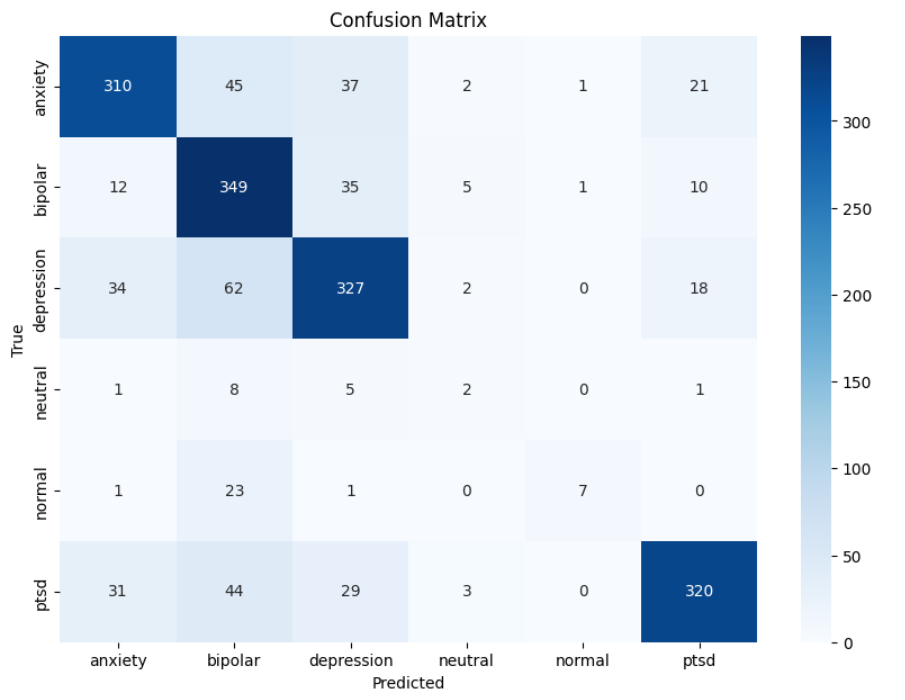
\includegraphics[width=1.0\textwidth]{Images/Confusion Matrix LR.png}  
    \caption{Confusion Matrix for Logistic Regression}
    \label{Project Modules}  % Label for referencing the figure
\end{figure}

\pagebreak
\textbf{Confusion Matrix Analysis:}

\begin{itemize}
    \item The confusion matrix reveals where the model misclassifies different categories. For example:
    \begin{itemize}
        \item \textbf{Anxiety} is often confused with \textbf{Bipolar} and \textbf{Depression}, indicating overlapping features between these classes.
        \item \textbf{PTSD} is more distinct, as shown by a higher number of true positive predictions (320), suggesting that the model can better differentiate this category.
    \end{itemize}
    \item Overall, the confusion matrix helps pinpoint specific classes where the model's predictions are less reliable, providing direction for further improvements.
\end{itemize}




\subsection{Results of K-Nearest Neighbors (KNN) and Hyperparameter Tuning}

\begin{center}
    KNN Classification Report (Before Hyperparameter Tuning)
\begin{tabular}{|l|c|c|c|c|}
\hline
\textbf{Class} & \textbf{Precision} & \textbf{Recall} & \textbf{F1-Score} & \textbf{Support} \\ \hline
Anxiety        & 0.60               & 0.36            & 0.45              & 416              \\ \hline
Bipolar        & 0.31               & 0.83            & 0.45              & 412              \\ \hline
Depression     & 0.46               & 0.35            & 0.40              & 443              \\ \hline
Neutral        & 0.00               & 0.00            & 0.00              & 17               \\ \hline
Normal         & 0.29               & 0.06            & 0.10              & 32               \\ \hline
PTSD           & 0.81               & 0.11            & 0.20              & 427              \\ \hline
\textbf{Accuracy} & \multicolumn{4}{|c|}{39.61\%} \\ \hline
\textbf{Macro Avg} & 0.41            & 0.28            & 0.27              & 1747             \\ \hline
\textbf{Weighted Avg} & 0.54         & 0.40            & 0.36              & 1747             \\ \hline
\end{tabular}


\vspace{0.25in}

Confusion Matrix for KNN (Before Hyperparameter Tuning)
\begin{tabular}{|l|c|c|c|c|c|c|}
\hline
\textbf{True Class} & \textbf{Anxiety} & \textbf{Bipolar} & \textbf{Depression} & \textbf{Neutral} & \textbf{Normal} & \textbf{PTSD} \\ \hline
Anxiety             & 148              & 221              & 46                  & 0                & 0               & 1             \\ \hline
Bipolar             & 24               & 340              & 42                  & 1                & 3               & 2             \\ \hline
Depression          & 36               & 246              & 154                 & 0                & 0               & 7             \\ \hline
Neutral             & 2                & 14               & 0                   & 0                & 0               & 1             \\ \hline
Normal              & 0                & 30               & 0                   & 0                & 2               & 0             \\ \hline
PTSD                & 38               & 248              & 91                  & 0                & 2               & 48            \\ \hline
\end{tabular}


\vspace{1.5in}

\pagebreak
KNN Classification Report (After Hyperparameter Tuning)
\begin{tabular}{|l|c|c|c|c|}
\hline
\textbf{Class} & \textbf{Precision} & \textbf{Recall} & \textbf{F1-Score} & \textbf{Support} \\ \hline
Anxiety        & 0.65               & 0.34            & 0.45              & 416              \\ \hline
Bipolar        & 0.32               & 0.82            & 0.46              & 412              \\ \hline
Depression     & 0.47               & 0.39            & 0.43              & 443              \\ \hline
Neutral        & 0.00               & 0.00            & 0.00              & 17               \\ \hline
Normal         & 0.26               & 0.19            & 0.22              & 32               \\ \hline
PTSD           & 0.73               & 0.15            & 0.24              & 427              \\ \hline
\textbf{Accuracy} & \multicolumn{4}{|c|}{41.27\%} \\ \hline
\textbf{Macro Avg} & 0.40            & 0.31            & 0.30              & 1747             \\ \hline
\textbf{Weighted Avg} & 0.53         & 0.41            & 0.39              & 1747             \\ \hline
\end{tabular}


\vspace{0.25in}

Confusion Matrix for KNN (After Hyperparameter Tuning)
\begin{tabular}{|l|c|c|c|c|c|c|}
\hline
\textbf{True Class} & \textbf{Anxiety} & \textbf{Bipolar} & \textbf{Depression} & \textbf{Neutral} & \textbf{Normal} & \textbf{PTSD} \\ \hline
Anxiety             & 143              & 214              & 52                  & 0                & 2               & 5             \\ \hline
Bipolar             & 19               & 337              & 45                  & 1                & 7               & 3             \\ \hline
Depression          & 31               & 223              & 173                 & 1                & 1               & 14            \\ \hline
Neutral             & 0                & 15               & 1                   & 0                & 0               & 1             \\ \hline
Normal              & 0                & 26               & 0                   & 0                & 6               & 0             \\ \hline
PTSD                & 28               & 233              & 97                  & 0                & 7               & 62            \\ \hline
\end{tabular}
\end{center}

\subsection{Explanations for KNN Results}

\begin{itemize}
    \item \textbf{Initial KNN Performance:}
    \begin{itemize}
        \item The initial accuracy of the KNN model is low (\textbf{39.61\%}), indicating that the model struggles to classify the mental health categories effectively.
        \item The recall for the \textbf{Bipolar} class is high (0.83), suggesting that the model is sensitive to detecting bipolar cases but tends to misclassify other categories as bipolar.
        \item Other classes like \textbf{Neutral} and \textbf{Normal} have very low precision and recall, highlighting the model’s inability to distinguish these less frequent categories.
    \end{itemize}

    \item \textbf{After Hyperparameter Tuning:}
    \begin{itemize}
        \item The accuracy improved slightly to \textbf{41.27\%} after tuning with the best hyperparameters \{'weights': 'distance', 'n\_neighbors': 4, 'metric': 'euclidean'\}, indicating minor gains in the classification.
        \item The recall for the \textbf{Anxiety} class decreased, while the precision increased, showing a trade-off in performance.
        \item For the \textbf{Depression} class, both precision and recall increased slightly, indicating that the tuning helped the model distinguish depression cases better.
    \end{itemize}

    \item \textbf{Confusion Matrix Analysis:}
    \begin{itemize}
        \item Many instances of \textbf{Anxiety} and \textbf{Depression} are misclassified as \textbf{Bipolar}, showing overlapping features between these classes.
        \item The class \textbf{PTSD} has a low recall, indicating that most of the PTSD samples are misclassified into other categories.
        \item The class distribution imbalance and similar feature patterns might be contributing to the misclassifications, causing the model to favor more common classes like Bipolar.
    \end{itemize}
\end{itemize}

\begin{figure}[h!]  
    \centering
    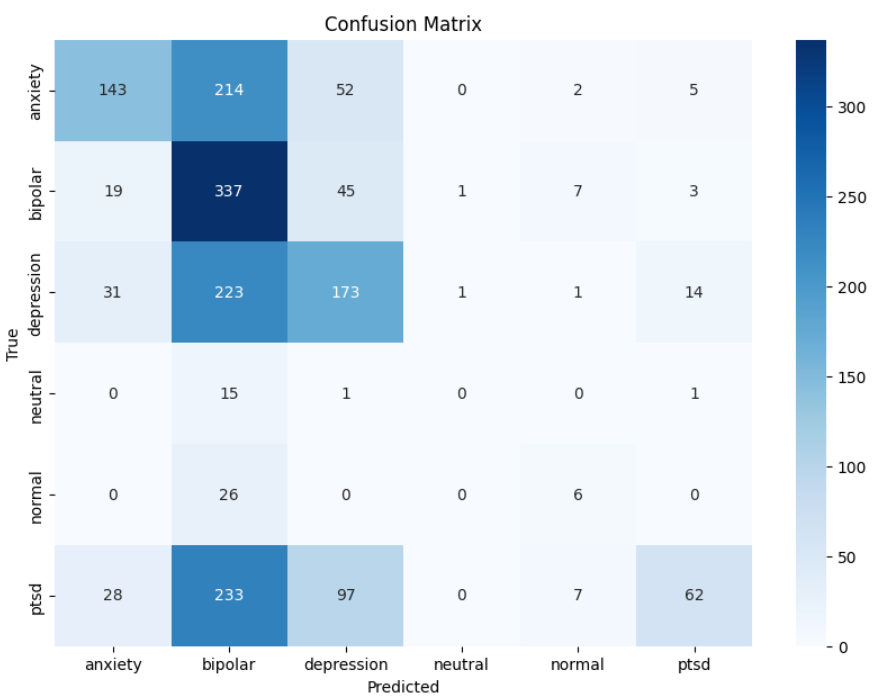
\includegraphics[width=1.0\textwidth]{Images/Confusion Matrix KNN.png}  
    \caption{Confusion Matrix for KNN}
    \label{Confusion Matrix KNN}  % Label for referencing the figure
\end{figure}

\pagebreak
\subsection{Results of Support Vector Machine (SVM) and Hyperparameter Tuning}

\begin{center}
    SVM Classification Report (Before Hyperparameter Tuning)
\begin{tabular}{|l|c|c|c|c|}
\hline
\textbf{Class} & \textbf{Precision} & \textbf{Recall} & \textbf{F1-Score} & \textbf{Support} \\ \hline
Anxiety        & 0.70               & 0.70            & 0.70              & 416              \\ \hline
Bipolar        & 0.65               & 0.81            & 0.72              & 412              \\ \hline
Depression     & 0.72               & 0.67            & 0.69              & 443              \\ \hline
Neutral        & 0.19               & 0.18            & 0.18              & 17               \\ \hline
Normal         & 0.62               & 0.25            & 0.36              & 32               \\ \hline
PTSD           & 0.81               & 0.71            & 0.76              & 427              \\ \hline
\textbf{Accuracy} & \multicolumn{4}{|c|}{70.75\%} \\ \hline
\textbf{Macro Avg} & 0.61            & 0.55            & 0.57              & 1747             \\ \hline
\textbf{Weighted Avg} & 0.71         & 0.71            & 0.71              & 1747             \\ \hline
\end{tabular}

\vspace{0.25in}

Confusion Matrix for SVM (Before Hyperparameter Tuning)
\begin{tabular}{|l|c|c|c|c|c|c|}
\hline
\textbf{True Class} & \textbf{Anxiety} & \textbf{Bipolar} & \textbf{Depression} & \textbf{Neutral} & \textbf{Normal} & \textbf{PTSD} \\ \hline
Anxiety             & 292              & 45               & 44                  & 2                & 1               & 32            \\ \hline
Bipolar             & 23               & 333              & 37                  & 5                & 3               & 11            \\ \hline
Depression          & 59               & 58               & 296                 & 2                & 0               & 28            \\ \hline
Neutral             & 1                & 7                & 5                   & 3                & 0               & 1             \\ \hline
Normal              & 0                & 24               & 0                   & 0                & 8               & 0             \\ \hline
PTSD                & 41               & 47               & 30                  & 4                & 1               & 304           \\ \hline
\end{tabular}

\vspace{0.25in}

SVM Classification Report (After Hyperparameter Tuning)
\begin{tabular}{|l|c|c|c|c|}
\hline
\textbf{Class} & \textbf{Precision} & \textbf{Recall} & \textbf{F1-Score} & \textbf{Support} \\ \hline
Anxiety        & 0.78               & 0.71            & 0.74              & 416              \\ \hline
Bipolar        & 0.61               & 0.83            & 0.70              & 412              \\ \hline
Depression     & 0.75               & 0.70            & 0.72              & 443              \\ \hline
Neutral        & 0.13               & 0.12            & 0.12              & 17               \\ \hline
Normal         & 0.57               & 0.12            & 0.21              & 32               \\ \hline
PTSD           & 0.84               & 0.71            & 0.77              & 427              \\ \hline
\textbf{Accuracy} & \multicolumn{4}{|c|}{72.07\%} \\ \hline
\textbf{Macro Avg} & 0.61            & 0.53            & 0.54              & 1747             \\ \hline
\textbf{Weighted Avg} & 0.73         & 0.72            & 0.72              & 1747             \\ \hline
\end{tabular}

\vspace{0.25in}

Confusion Matrix for SVM (After Hyperparameter Tuning)
\begin{tabular}{|l|c|c|c|c|c|c|}
\hline
\textbf{True Class} & \textbf{Anxiety} & \textbf{Bipolar} & \textbf{Depression} & \textbf{Neutral} & \textbf{Normal} & \textbf{PTSD} \\ \hline
Anxiety             & 292              & 45               & 44                  & 2                & 1               & 32            \\ \hline
Bipolar             & 23               & 333              & 37                  & 5                & 3               & 11            \\ \hline
Depression          & 59               & 58               & 296                 & 2                & 0               & 28            \\ \hline
Neutral             & 1                & 7                & 5                   & 3                & 0               & 1             \\ \hline
Normal              & 0                & 24               & 0                   & 0                & 8               & 0             \\ \hline
PTSD                & 41               & 47               & 30                  & 4                & 1               & 304           \\ \hline
\end{tabular}
\end{center}

\subsection{Explanations for SVM Results}

\begin{itemize}
    \item \textbf{Initial SVM Performance:}
    \begin{itemize}
        \item The initial accuracy of the SVM model is \textbf{70.75\%}, indicating a moderate performance in classifying mental health categories.
        \item The \textbf{Bipolar} class has a high recall of 0.81, indicating the model's ability to identify most bipolar cases correctly. However, the precision is lower, showing misclassification with other classes.
        \item The \textbf{Neutral} and \textbf{Normal} classes have low precision and recall values, indicating that the model struggles to identify these minority classes.
    \end{itemize}

    \item \textbf{After Hyperparameter Tuning:}
    \begin{itemize}
        \item The accuracy improved slightly to \textbf{72.07\%} with the best hyperparameters \{'kernel': 'linear', 'gamma': 'scale', 'C': 0.1\}.
        \item The recall for the \textbf{Anxiety} and \textbf{Depression} classes increased, indicating better sensitivity to these categories.
        \item The precision for \textbf{PTSD} also improved, suggesting the model has a clearer distinction for this class after tuning.
    \end{itemize}

    \begin{figure}[h!]  
    \centering
    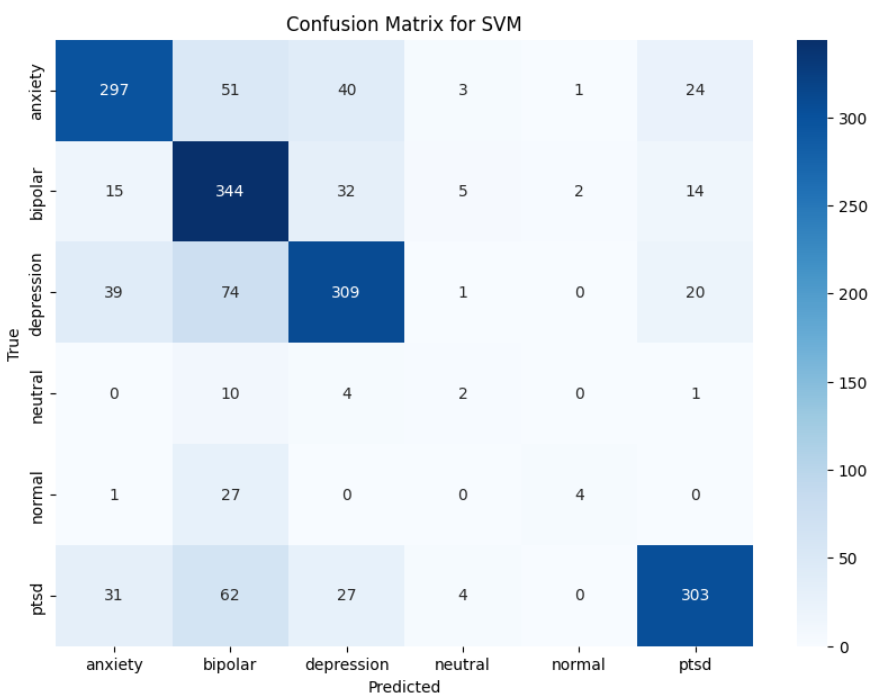
\includegraphics[width=0.8\textwidth]{Images/Confusion Matrix SVM.png}  
    \caption{Confusion Matrix for SVM}
    \label{Confusion Matrix SVM}  % Label for referencing the figure
    \end{figure}

    \item \textbf{Confusion Matrix Analysis:}
    \begin{itemize}
        \item Many instances of \textbf{Anxiety} and \textbf{Depression} are misclassified as \textbf{Bipolar}, showing overlapping features between these classes.
        \item The \textbf{Neutral} and \textbf{Normal} classes have very few true positive predictions, indicating that the SVM model still struggles to capture these less frequent categories.
        \item Overall, the slight improvement in performance after hyperparameter tuning suggests that tuning helped the SVM classifier better balance the trade-offs between precision and recall for most major classes.
    \end{itemize}
\end{itemize}



\subsection{Results of Naive Bayes and Hyperparameter Tuning}

\begin{center}
    Naive Bayes Classification Report (Before Hyperparameter Tuning)
\begin{tabular}{|l|c|c|c|c|}
\hline
\textbf{Class} & \textbf{Precision} & \textbf{Recall} & \textbf{F1-Score} & \textbf{Support} \\ \hline
Anxiety        & 0.69               & 0.72            & 0.70              & 416              \\ \hline
Bipolar        & 0.79               & 0.56            & 0.65              & 412              \\ \hline
Depression     & 0.65               & 0.82            & 0.72              & 443              \\ \hline
Neutral        & 0.17               & 0.29            & 0.21              & 17               \\ \hline
Normal         & 0.14               & 0.03            & 0.05              & 32               \\ \hline
PTSD           & 0.73               & 0.72            & 0.72              & 427              \\ \hline
\textbf{Accuracy} & \multicolumn{4}{|c|}{68.92\%} \\ \hline
\textbf{Macro Avg} & 0.53            & 0.52            & 0.51              & 1747             \\ \hline
\textbf{Weighted Avg} & 0.70         & 0.69            & 0.68              & 1747             \\ \hline
\end{tabular}

\vspace{0.25in}

Confusion Matrix for Naive Bayes (Before Hyperparameter Tuning)
\begin{tabular}{|l|c|c|c|c|c|c|}
\hline
\textbf{True Class} & \textbf{Anxiety} & \textbf{Bipolar} & \textbf{Depression} & \textbf{Neutral} & \textbf{Normal} & \textbf{PTSD} \\ \hline
Anxiety             & 300              & 14               & 61                  & 8                & 3               & 30            \\ \hline
Bipolar             & 51               & 229              & 78                  & 5                & 0               & 49            \\ \hline
Depression          & 27               & 20               & 362                 & 5                & 1               & 28            \\ \hline
Neutral             & 1                & 6                & 4                   & 5                & 1               & 0             \\ \hline
Normal              & 12               & 2                & 9                   & 1                & 1               & 7             \\ \hline
PTSD                & 46               & 20               & 47                  & 6                & 1               & 307           \\ \hline
\end{tabular}

\vspace{0.25in}

Naive Bayes Classification Report (After Hyperparameter Tuning)
\begin{tabular}{|l|c|c|c|c|}
\hline
\textbf{Class} & \textbf{Precision} & \textbf{Recall} & \textbf{F1-Score} & \textbf{Support} \\ \hline
Anxiety        & 0.68               & 0.74            & 0.71              & 277              \\ \hline
Bipolar        & 0.77               & 0.63            & 0.69              & 289              \\ \hline
Depression     & 0.69               & 0.81            & 0.74              & 316              \\ \hline
Neutral        & 0.20               & 0.43            & 0.27              & 14               \\ \hline
Normal         & 0.17               & 0.04            & 0.07              & 23               \\ \hline
PTSD           & 0.75               & 0.69            & 0.72              & 304              \\ \hline
\textbf{Accuracy} & \multicolumn{4}{|c|}{70.16\%} \\ \hline
\textbf{Macro Avg} & 0.54            & 0.56            & 0.53              & 1223             \\ \hline
\textbf{Weighted Avg} & 0.71         & 0.70            & 0.70              & 1223             \\ \hline
\end{tabular}

\vspace{0.25in}

Confusion Matrix for Naive Bayes (After Hyperparameter Tuning)
\begin{tabular}{|l|c|c|c|c|c|c|}
\hline
\textbf{True Class} & \textbf{Anxiety} & \textbf{Bipolar} & \textbf{Depression} & \textbf{Neutral} & \textbf{Normal} & \textbf{PTSD} \\ \hline
Anxiety             & 300              & 14               & 61                  & 8                & 3               & 30            \\ \hline
Bipolar             & 51               & 229              & 78                  & 5                & 0               & 49            \\ \hline
Depression          & 27               & 20               & 362                 & 5                & 1               & 28            \\ \hline
Neutral             & 1                & 6                & 4                   & 5                & 1               & 0             \\ \hline
Normal              & 12               & 2                & 9                   & 1                & 1               & 7             \\ \hline
PTSD                & 46               & 20               & 47                  & 6                & 1               & 307           \\ \hline
\end{tabular}    
\end{center}

\subsection{Explanations for Naive Bayes Results}

\begin{itemize}
    \item \textbf{Initial Naive Bayes Performance:}
    \begin{itemize}
        \item The initial accuracy of the Naive Bayes model is \textbf{68.92\%}, indicating moderate classification performance.
        \item The \textbf{Anxiety} and \textbf{Depression} classes have relatively higher recall values, suggesting that the model is sensitive to identifying these categories correctly.
        \item The \textbf{Neutral} and \textbf{Normal} classes have very low precision and recall, indicating that the model struggles to classify these minority classes.
    \end{itemize}

    \item \textbf{After Hyperparameter Tuning:}
    \begin{itemize}
        \item The accuracy increased slightly to \textbf{70.16\%} with the best hyperparameters \{'fit\_prior': True, 'alpha': 0.5\}, showing a minor performance improvement.
        \item The recall for the \textbf{Anxiety} and \textbf{Depression} classes increased, indicating better sensitivity and improved classification for these classes.
        \item However, the precision for the \textbf{Bipolar} class decreased slightly, suggesting a trade-off in correctly identifying true positive cases for this class.
    \end{itemize}
    
    \item \textbf{Confusion Matrix Analysis:}
    \begin{itemize}
        \item Many instances of \textbf{Anxiety} and \textbf{Depression} are misclassified as \textbf{Bipolar}, indicating overlapping feature characteristics between these categories.
        \item The \textbf{Neutral} and \textbf{Normal} classes continue to have very few true positive predictions, highlighting the model’s struggle to capture these less frequent categories.
        \item The increase in recall for major classes like \textbf{Anxiety} and \textbf{Depression} after tuning suggests that the model learned better class-specific distributions.
    \end{itemize}
\end{itemize}

 \begin{figure}[h!]  
    \centering
    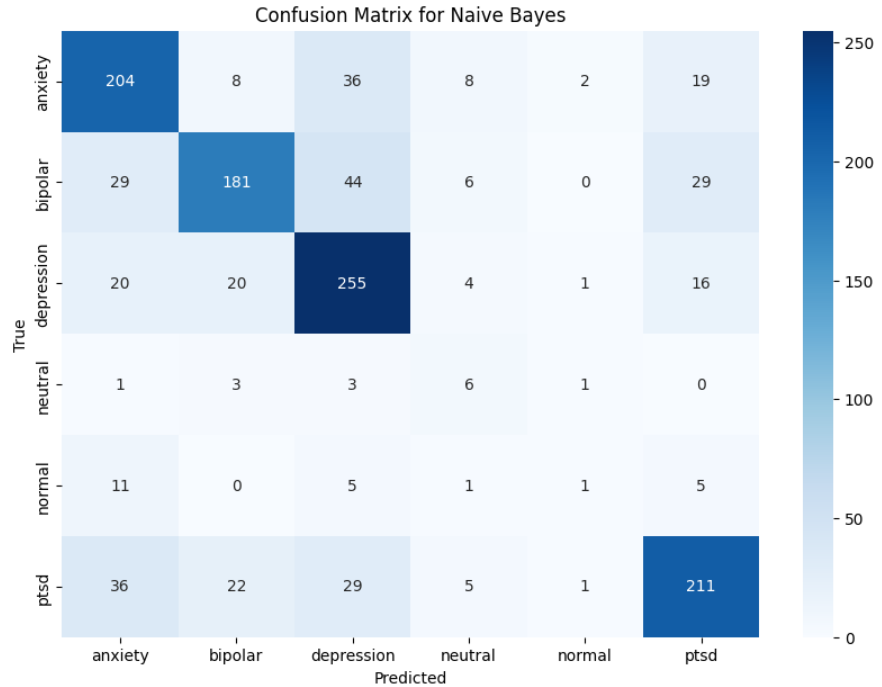
\includegraphics[width=0.8\textwidth]{Images/Confusion Matrix NB.png}  
    \caption{Confusion Matrix for Naive Bayes}
    \label{Confusion Matrix NB}  % Label for referencing the figure
    \end{figure}

\subsection{Results of Random Forest and Hyperparameter Tuning}

\begin{center}
    Random Forest Classification Report
\begin{tabular}{|l|c|c|c|c|}
\hline
\textbf{Class} & \textbf{Precision} & \textbf{Recall} & \textbf{F1-Score} & \textbf{Support} \\ \hline
Anxiety        & 0.76               & 0.77            & 0.76              & 416              \\ \hline
Bipolar        & 0.70               & 0.77            & 0.74              & 412              \\ \hline
Depression     & 0.69               & 0.80            & 0.74              & 443              \\ \hline
Neutral        & 0.20               & 0.06            & 0.09              & 17               \\ \hline
Normal         & 0.83               & 0.16            & 0.26              & 32               \\ \hline
PTSD           & 0.88               & 0.73            & 0.80              & 427              \\ \hline
\textbf{Accuracy} & \multicolumn{4}{|c|}{74.87\%} \\ \hline
\textbf{Macro Avg} & 0.68            & 0.55            & 0.57              & 1747             \\ \hline
\textbf{Weighted Avg} & 0.75         & 0.75            & 0.74              & 1747             \\ \hline
\end{tabular}

\vspace{0.25in}

Confusion Matrix for Random Forest
\begin{tabular}{|l|c|c|c|c|c|c|}
\hline
\textbf{True Class} & \textbf{Anxiety} & \textbf{Bipolar} & \textbf{Depression} & \textbf{Neutral} & \textbf{Normal} & \textbf{PTSD} \\ \hline
Anxiety             & 319              & 38               & 50                  & 0                & 0               & 9             \\ \hline
Bipolar             & 23               & 319              & 53                  & 2                & 1               & 14            \\ \hline
Depression          & 31               & 41               & 353                 & 0                & 0               & 18            \\ \hline
Neutral             & 1                & 9                & 5                   & 1                & 0               & 1             \\ \hline
Normal              & 3                & 24               & 0                   & 0                & 5               & 0             \\ \hline
PTSD                & 43               & 22               & 49                  & 2                & 0               & 311           \\ \hline
\end{tabular}    
\end{center}

\subsection{Explanations for Random Forest Results}

\begin{itemize}
    \item \textbf{Overall Performance:}
    \begin{itemize}
        \item The accuracy of the Random Forest model is \textbf{74.87\%}, indicating a good level of performance in classifying the different mental health categories.
        \item The \textbf{PTSD} class shows the highest precision (0.88) and recall (0.73), suggesting that the model is effective at identifying PTSD cases correctly.
    \end{itemize}

    \item \textbf{Class-wise Analysis:}
    \begin{itemize}
        \item The precision and recall for the \textbf{Anxiety} and \textbf{Depression} classes are reasonably balanced, indicating that the model is adept at classifying these categories.
        \item The \textbf{Bipolar} class has a slightly lower precision but high recall, suggesting that while the model can identify bipolar instances effectively, it also misclassifies some non-bipolar cases as bipolar.
        \item The performance for the \textbf{Neutral} and \textbf{Normal} classes is concerning, with very low recall and F1-scores, indicating that these classes are often misclassified.
    \end{itemize}

    \begin{figure}[h!]  
    \centering
    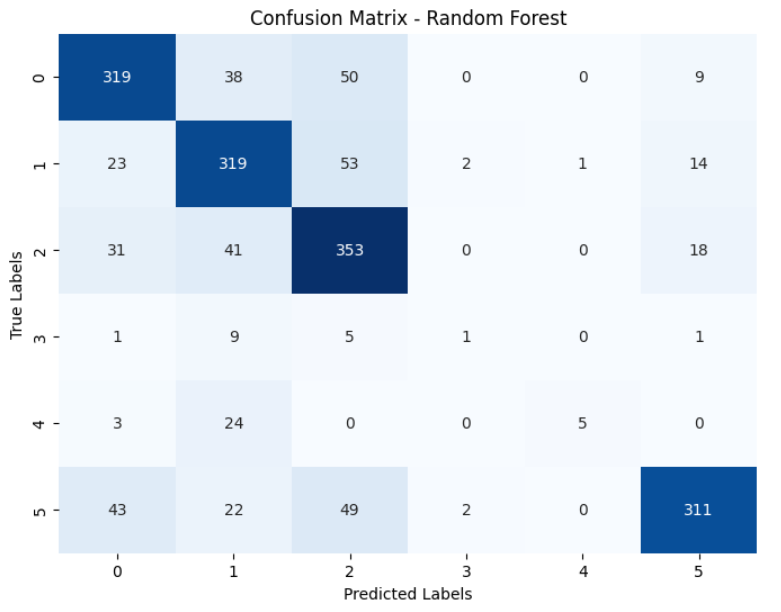
\includegraphics[width=0.9\textwidth]{Images/Confusion Matrix RF.png}  
    \caption{Confusion Matrix for Random Forest}
    \label{Confusion Matrix RF}  % Label for referencing the figure
    \end{figure}

    \item \textbf{Confusion Matrix Analysis:}
    \begin{itemize}
        \item The confusion matrix reveals that many instances of \textbf{Anxiety} and \textbf{Depression} are correctly classified, with a significant number of \textbf{Neutral} instances being misclassified.
        \item The low count for \textbf{Normal} indicates that the model has trouble distinguishing this category, as evidenced by the high number of false positives.
        \item The high number of true positive predictions for \textbf{PTSD} (311) suggests that the Random Forest model is effective in distinguishing PTSD from other classes, likely due to its ability to handle complex feature interactions well.
    \end{itemize}
\end{itemize}

\subsection{Comparison of Different Models}

\begin{center}
    \centering
    Datasets Overview \\
    \vspace{0.05in}
    \begin{tabular}{|l|c|c|c|}
    \hline
    \textbf{Dataset} & \textbf{Capacity} & \textbf{Modality} \\ \hline
    Dataset - Reddit  & 12000              & Single            \\ \hline
    Dataset - Twitter  & 900                & Single            \\ \hline
    DS - Reddit + Twitter & 12900          & Single            \\ \hline
    \end{tabular}

    \vspace{0.25in}

\centering
Comparison of Classification Metrics for Anxiety
\begin{tabular}{|l|c|c|c|c|}
\hline
\textbf{Model} & \textbf{Precision} & \textbf{Recall} & \textbf{F1-Score} & \textbf{Support} \\ \hline
Logistic Regression & 0.78 & 0.73 & 0.75 & 416 \\ \hline
KNN                & 0.60 & 0.36 & 0.45 & 416 \\ \hline
SVM                & 0.70 & 0.70 & 0.70 & 416 \\ \hline
Naive Bayes        & 0.69 & 0.72 & 0.70 & 416 \\ \hline
Random Forest      & 0.76 & 0.77 & 0.76 & 416 \\ \hline
\end{tabular}

\vspace{0.25in}

\centering
Comparison of Classification Metrics for Bipolar
\begin{tabular}{|l|c|c|c|c|}
\hline
\textbf{Model} & \textbf{Precision} & \textbf{Recall} & \textbf{F1-Score} & \textbf{Support} \\ \hline
Logistic Regression & 0.66 & 0.84 & 0.74 & 412 \\ \hline
KNN                & 0.31 & 0.83 & 0.45 & 412 \\ \hline
SVM                & 0.65 & 0.81 & 0.72 & 412 \\ \hline
Naive Bayes        & 0.79 & 0.56 & 0.65 & 412 \\ \hline
Random Forest      & 0.70 & 0.77 & 0.74 & 412 \\ \hline
\end{tabular}

\vspace{0.25in}

\centering
Comparison of Classification Metrics for Depression
\begin{tabular}{|l|c|c|c|c|}
\hline
\textbf{Model} & \textbf{Precision} & \textbf{Recall} & \textbf{F1-Score} & \textbf{Support} \\ \hline
Logistic Regression & 0.74 & 0.72 & 0.73 & 443 \\ \hline
KNN                & 0.46 & 0.35 & 0.40 & 443 \\ \hline
SVM                & 0.72 & 0.67 & 0.69 & 443 \\ \hline
Naive Bayes        & 0.65 & 0.82 & 0.72 & 443 \\ \hline
Random Forest      & 0.69 & 0.80 & 0.74 & 443 \\ \hline
\end{tabular}

\vspace{0.25in}

\centering
Comparison of Classification Metrics for Neutral
\begin{tabular}{|l|c|c|c|c|}
\hline
\textbf{Model} & \textbf{Precision} & \textbf{Recall} & \textbf{F1-Score} & \textbf{Support} \\ \hline
Logistic Regression & 0.08 & 0.06 & 0.07 & 17 \\ \hline
KNN                & 0.00 & 0.00 & 0.00 & 17 \\ \hline
SVM                & 0.19 & 0.18 & 0.18 & 17 \\ \hline
Naive Bayes        & 0.17 & 0.29 & 0.21 & 17 \\ \hline
Random Forest      & 0.20 & 0.06 & 0.09 & 17 \\ \hline
\end{tabular}


\vspace{0.25in}

Comparison of Classification Metrics for Normal
\begin{tabular}{|l|c|c|c|c|}
\hline
\textbf{Model} & \textbf{Precision} & \textbf{Recall} & \textbf{F1-Score} & \textbf{Support} \\ \hline
Logistic Regression & 0.78 & 0.22 & 0.34 & 32 \\ \hline
KNN                & 0.29 & 0.06 & 0.10 & 32 \\ \hline
SVM                & 0.62 & 0.25 & 0.36 & 32 \\ \hline
Naive Bayes        & 0.14 & 0.03 & 0.05 & 32 \\ \hline
Random Forest      & 0.83 & 0.16 & 0.26 & 32 \\ \hline
\end{tabular}

\vspace{0.25in}
Comparison of Classification Metrics for PTSD
\begin{tabular}{|l|c|c|c|c|}
\hline
\textbf{Model} & \textbf{Precision} & \textbf{Recall} & \textbf{F1-Score} & \textbf{Support} \\ \hline
Logistic Regression & 0.83 & 0.74 & 0.78 & 427 \\ \hline
KNN                & 0.81 & 0.11 & 0.20 & 427 \\ \hline
SVM                & 0.81 & 0.71 & 0.76 & 427 \\ \hline
Naive Bayes        & 0.73 & 0.72 & 0.72 & 427 \\ \hline
Random Forest      & 0.88 & 0.73 & 0.80 & 427 \\ \hline
\end{tabular}

\vspace{0.25in}
Comparison of Classification Metrics for Anxiety (After Hyperparameter Tuning)
\begin{tabular}{|l|c|c|c|c|}
\hline
\textbf{Model} & \textbf{Precision} & \textbf{Recall} & \textbf{F1-Score} & \textbf{Support} \\ \hline
Logistic Regression & 0.80 & 0.75 & 0.77 & 416 \\ \hline
KNN                & 0.65 & 0.34 & 0.45 & 416 \\ \hline
SVM                & 0.78 & 0.71 & 0.74 & 416 \\ \hline
Naive Bayes        & 0.68 & 0.74 & 0.71 & 277 \\ \hline
\end{tabular}

\vspace{0.25in}

Comparison of Classification Metrics for Bipolar (After Hyperparameter Tuning)
\begin{tabular}{|l|c|c|c|c|}
\hline
\textbf{Model} & \textbf{Precision} & \textbf{Recall} & \textbf{F1-Score} & \textbf{Support} \\ \hline
Logistic Regression & 0.66 & 0.85 & 0.74 & 412 \\ \hline
KNN                & 0.32 & 0.82 & 0.46 & 412 \\ \hline
SVM                & 0.61 & 0.83 & 0.70 & 412 \\ \hline
Naive Bayes        & 0.77 & 0.63 & 0.69 & 289 \\ \hline
\end{tabular}

\vspace{0.25in}

Comparison of Classification Metrics for Depression (After Hyperparameter Tuning)
\begin{tabular}{|l|c|c|c|c|}
\hline
\textbf{Model} & \textbf{Precision} & \textbf{Recall} & \textbf{F1-Score} & \textbf{Support} \\ \hline
Logistic Regression & 0.75 & 0.74 & 0.75 & 443 \\ \hline
KNN                & 0.47 & 0.39 & 0.43 & 443 \\ \hline
SVM                & 0.75 & 0.70 & 0.72 & 443 \\ \hline
Naive Bayes        & 0.69 & 0.81 & 0.74 & 316 \\ \hline
\end{tabular}

\vspace{0.25in}

Comparison of Classification Metrics for Neutral (After Hyperparameter Tuning)
\begin{tabular}{|l|c|c|c|c|}
\hline
\textbf{Model} & \textbf{Precision} & \textbf{Recall} & \textbf{F1-Score} & \textbf{Support} \\ \hline
Logistic Regression & 0.14 & 0.12 & 0.13 & 17 \\ \hline
KNN                & 0.00 & 0.00 & 0.00 & 17 \\ \hline
SVM                & 0.13 & 0.12 & 0.12 & 17 \\ \hline
Naive Bayes        & 0.20 & 0.43 & 0.27 & 14 \\ \hline
\end{tabular}

\vspace{0.25in}
Comparison of Classification Metrics for Normal (After Hyperparameter Tuning)
\begin{tabular}{|l|c|c|c|c|}
\hline
\textbf{Model} & \textbf{Precision} & \textbf{Recall} & \textbf{F1-Score} & \textbf{Support} \\ \hline
Logistic Regression & 0.78 & 0.22 & 0.34 & 32 \\ \hline
KNN                & 0.26 & 0.19 & 0.22 & 32 \\ \hline
SVM                & 0.57 & 0.12 & 0.21 & 32 \\ \hline
Naive Bayes        & 0.17 & 0.04 & 0.07 & 23 \\ \hline
\end{tabular}

\vspace{0.25in}
Comparison of Classification Metrics for PTSD (After Hyperparameter Tuning)
\begin{tabular}{|l|c|c|c|c|}
\hline
\textbf{Model} & \textbf{Precision} & \textbf{Recall} & \textbf{F1-Score} & \textbf{Support} \\ \hline
Logistic Regression & 0.86 & 0.75 & 0.80 & 427 \\ \hline
KNN                & 0.73 & 0.15 & 0.24 & 427 \\ \hline
SVM                & 0.84 & 0.71 & 0.77 & 427 \\ \hline
Naive Bayes        & 0.75 & 0.69 & 0.72 & 304 \\ \hline
\end{tabular}

\end{center}


% ------------------------ Result and Analysis Ends -------------------------
